\chapter{Methodology \& Numerical Simulation}
\label{ch:numsim}

% Brief summation of computational work

% Why is this it's own chapter?

% Breakdown of chapter, what this involves

\section{A Short History of Numerical simulations}
\label{sec:numsim}

% A short history of computational fluid dynamics



\section{The Purpose of Numerical Simulations}
\label{sec:numerical-purpose}

% Why are they useful in general



% Why are they useful in the context of a colliding wind binary problem

Numerical simulations, due to 

% Why are colliding wind binary systems such a pain to solve

\section{The Mathematics of Numerical Simulations}
\label{sec:numerical-math}

% Numerical solvers/Riemann problems

% Godunov method

% Pier

% Numerical integration

%% Strong stability preserving methods

\section{Computational Hydrodynamics}
\label{sec:hydrodynamics}

\subsection{Comparison of hydrodynamical methods}

% This section will cover hydrodynamical solvers, a brief history of the problem, cover the lineage of 

% briefly cover MG hydrodynamical code, since this was used for the first half of this work before adopting a more modern hydro code

\section{The Athena++ Hydrodynamical code}
\label{sec:athenapp}

% General schema

% Meshblock system

% Refinement

This is covered in more detail in the next section (section \ref{sec:refinement}).

% Multi-core and parallelisation

Athena++ is highly parallel and utilises the OpenMP and OpenMPI software libraries in order \footnote{Sadly, the engineers at Intel who worked on the Netburst architecture were \href{https://web.archive.org/web/20210412001459/https://www.anandtech.com/show/680/6}{wrong}, processors can't easily scale up to dozens of \si{\giga\hertz}, instead, multiple cores have to be used, making high performance code that much harder to write.}
%
Meshblocks are distributed to processor cores 
% OpenMPI
In the case of a simulation that requires more cores than a single computer can provide, OpenMPI is used to distribute meshblocks between nodes in a HPC\footnote{High Performance Compute} cluster, whilst this can introduce bottlenecks due to the comparatively slow networking between nodes, this allows for thousands of cores to be used, rather than dozens.
% Both in concert

% Ghost cells
In order to prevent numerical errors from occurring between the interfaces between meshblocks, ``ghost cells'', cells from adjacent meshblocks copied into the current meshblock, are used.
%//TODO this needs some work

% Briefly discuss parallel performance


\section{Mesh Refinement}
\label{sec:refinement}

One of the problems previously discussed with modelling CWB systems is the 

%//TODO include a diagram of 

\begin{figure}
  \centering
  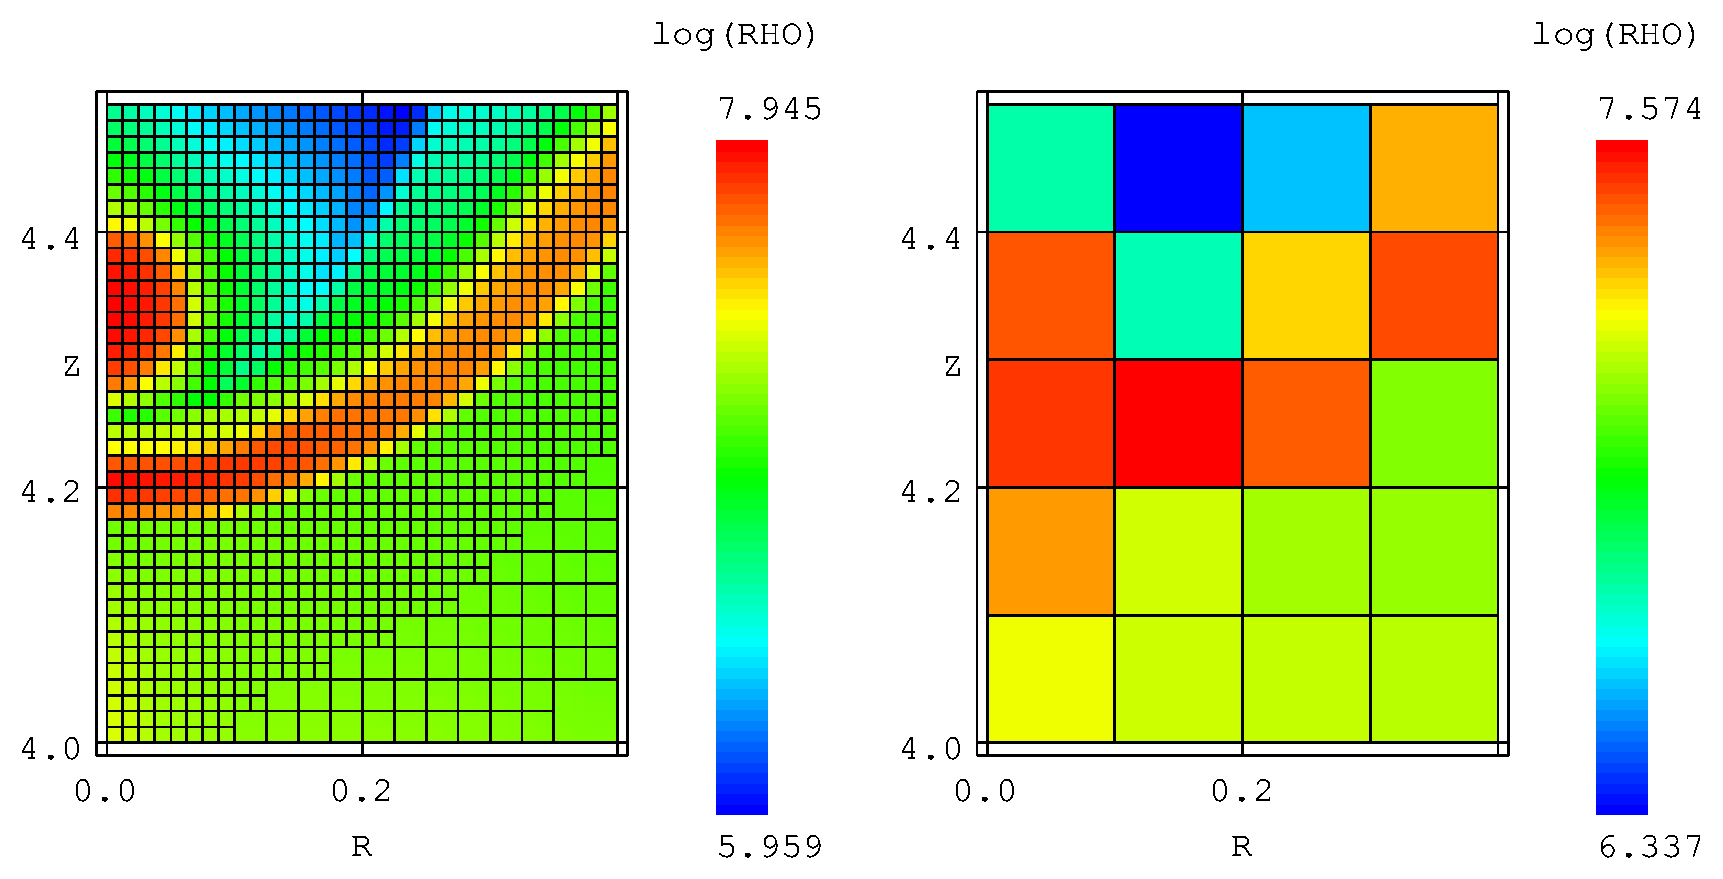
\includegraphics[width=5in]{assets/mergecellc.pdf}
  \caption[Adaptive mesh refinement comparison]{An example of adaptive mesh refinement in the \texttt{MG} hydrodynamical code around the OB star in a colliding wind binary problem using cylindrically symmetric co-ordinates. With AMR the region is properly resolved, while without the system cannot adequately resolve the collision region.}
  \label{fig:mgrefine}
\end{figure}

The pseudocode for the refinement condition 

%//TODO these may need to be converted into more readable pseudocode, maybe a flow diagram?

\begin{lstlisting}[language=C++]
// Get cell width
Real dx = pmb->pcoord->dx1v(0);
// March through cells in block, checking distance from star to cell
for (int n = 0; n < NWIND; n++) {
  for (int k = pmb->ks; k <= pmb->ke; k++) {
    // Get Z co-ordinate separation from star
    Real zc  = pmb->pcoord->x3v(k) - star[n].pos[2];
    Real zc2 = SQR(zc);
    for (int j = pmb->js; j <= pmb->je; j++) {
      // Get Y co-ordinate separation from star
      Real yc  = pmb->pcoord->x2v(j) - star[n].pos[1];
      Real yc2 = SQR(yc);
      for (int i = pmb->is; i <= pmb->ie; i++) {
        // Get X co-ordinate separation from star
        Real xc  = pmb->pcoord->x1v(i) - star[n].pos[0];
        Real xc2 = SQR(xc);
        // Get radial distance from current star to cell
        Real r2 = xc2 + yc2 + zc2;
        Real r  = sqrt(r2);
        // Get approximate number of cells distance
        int ri = int(r/dx);
        // If number of cells distance is below threshold, refine
        if (ri < amr.star_separation) {
          return 1;
        }
      }
    }
  }
}
\end{lstlisting}

\begin{lstlisting}[language=c++]
// Check to see if meshblock contains the stagnation point
for (int k = pmb->ks; k <= pmb->ke; k++) {
  // Get Z co-ordinate separation from stagnation point
  Real zc  = pmb->pcoord->x3v(k) - wcr.pos[2];
  Real zc2 = SQR(zc);
  for (int j = pmb->js; j <= pmb->je; j++) {
    // Get Y co-ordinate separation from stagnation point
    Real yc  = pmb->pcoord->x2v(j) - wcr.pos[1];
    Real yc2 = SQR(yc);
    for (int i = pmb->is; i <= pmb->ie; i++) {
      // Get X co-ordinate separation from stagnation point
      Real xc  = pmb->pcoord->x1v(i) - wcr.pos[0];
      Real xc2 = SQR(xc);
      // Get radial distance to current cell
      Real r2 = xc2 + yc2 + zc2;
      Real r  = sqrt(r2);
      // Get approximate number of cells between cell and stagnation point
      int ri = int(r/dx);
      // If number of cells distance is below threshold, refine
      if (ri < amr.wcr_separation) {
        return 1;
      }
    }
  }
}
\end{lstlisting}

All cells that do not meet these criteria are flagged for de-refinement.

\section{Visualisation}

%//TODO section might not be necessary
Data was plotted using a series of custom programmes designed to parse data as quickly as possible, 
the Python plotting library provided in the Athena++ repository was modified to incorporate Delaunay triangulation, instead of interpolating data due to mesh refinement, data-points are triangulated with each other.
For 3D visualisation the VisIt data visualisation tool is used.

\section{Simulating CWB systems}

% Recap why CWB simulations are so complex 


% How is this performed, processes involved in mapping wind on stars, orbits, how these are performed in the context of athena++ or numsim in general

\subsection{Assumptions}

% Short subsection covering assumptions used in this project

% Wind mapping, lack of radiative line driving

% Radiation processes

% Short coverage on dust model, this is explained further in a alter section

\section{Cooling in numerical simulations}

% Brief recamp on radiative cooling processes, compare with physical section, why they are important in the context of our work
As discussed in section \ref{sec:wcrcooling}, there are many cooling processes that need to be considered when simulating a complex system such as a CWB.

Sufficient cooling is in fact, essential to this dust formation process.
Gas temperature in the immediate post-shock region can exceed $10^8\, \si{\kelvin}$, far beyond the temperatures required to adequately form dust, as any nascent grains would quickly be shattered by thermal processes.
There is sufficient evidence to suggest that significant, rapid temperature loss occurs in the post-shock regime, the high metallicity of the WC wind and high number density of atoms and ions makes it the ideal region for rapid cooling due to radiative processes.

% Why even include cooling
Another boundary to dust formation due to an insufficiently radiative post-shock flow is a lack of sufficient downstream density.
In the case of strong, adiabatic shocks, constraints are set on the downstream gas parameters of the system, such that:

\begin{subequations}
  \begin{align}
    u_b    & = \frac{1}{4} u_a , \\
    \rho_b & = 4 \rho_a , \\ 
    P_b    & = \frac{3}{4} \rho_a u_a^2 ,
  \end{align}
\end{subequations}

\noindent
where $a$ is the upstream side and $b$ is the downstream, post-shock side.
As the gas density can only be a factor of 4 larger than the post-shock flow, the post shock density (even if it were at  temperatures suitable for dust formation) is insufficiently dense for sufficient dust production.
However, in a radiative shock behaving isothermally (where the temperature change, $\Delta T$ throughout the entire lifespan of the fluid is equal to zero), the final density, $\rho_f$ can be approximated to:

\begin{equation}
  \rho_f \approx \gamma M_a^2 \rho_a,
\end{equation}

\noindent
where $M_a$ is the pre-shock mach number.
For a shock with an initial sound speed of $M_a = 100$ the final density can exceed the pre-shock density by a factor of $10^4$!

% Complexities, conservation, that kind of thing

Performing radiative cooling within a numerical simulation is computationally difficult, and trade-offs between accuracy and performance must be considered at every step of designing the simulation, as every single cell must undergo cooling.
For this project, the final cooling can be out by a few percent at worst, but is fast enough to run the simulations in a reasonable amount of time without excessive memory requirements.
In order to simplify the radiation calculations, radiation does not re-interact with the simulation, instead it is completely removed from the simulation.
Due to this, scattering, re-adsorption and radiative transfer are not simulated at all.\footnote{If these are considered, your programme is now a ray-tracing programme as well as a hydrodynamical code, which is its own, even more complicated field.}.
Other methods of reducing computational cost and optimising the code are used in this project, and will be described in detail in this section.

\subsection{Plasma cooling}

% This isn't a section on the radiative processeses themselves, but more to do with how plasma cooling is simulated 

% Mention stuff like MEKAL

% Use of a lookup table
Thus, instead of calculating the emissivity of the plasma for the current density, temperature and abundances, a lookup table is pre-calculated and loaded into the simulation at runtime.
These lookup tables are generated by combining a series of lookup tables generated for pure flows of elements, and combined based on the abundance of the element within the stellar wind, hence each star in the simulation has its own unique lookup table.
A typical lookup table in this project utilises logarithmically spaced temperature bins from $10^4\,\si{\kelvin}$ to $10^9\,\si{\kelvin}$, with 100 bins in total, if the calculated temperature is between bins a linear interpolation step is used to improve the accuracy of the the emissivity solution.
In order to calculate the energy loss within a cell, the following formulae is used:

\begin{equation}
  \frac{dE}{dt} = \left(\frac{\rho}{m_H}\right) \Lambda_w (T) ,
\end{equation}

\noindent
where $\Lambda_w(T)$ is the normalised emissivity at the cell temperature, T.
This solution is orders of magnitude faster than performing an emissivity calculation in every cell, and is essential to performing fast hydrodynamical simulations with plasma radiative cooling.

% Mean molecular mass


% Improvements to accuracy of lookup table, linear search
Other optimisations relied on replacing a na\"ive linear search with an indexing method that relied on the logarithmic spacing of the temperature bins, instead of performing a search the index, $n$, of the emissivity value stored in an array can be calculated using the formulae

\begin{equation}
    n = \left \lfloor \frac{\log(T) - \log(T)_\text{min}}{\delta \log (T)} \right \rfloor ,
\end{equation}

\noindent
where $\log(T)$ is the log of the cell temperature, $\log (T)_\text{min}$ is the minimum log temperature in the lookup table and $\delta \log (T)$ is the log spacing of the temperature bins. 
This speed-up is fairly significant as the average search performance changes from $\mathcal{O}(n)$ to $\mathcal{O}(1)$ time, a marked improvement over even a binary search, which would resolve in an average of $\mathcal{O}(\log n)$ time.
In the case of a 100 bin array this is only a minor speed-up, but with the sheer number of calculations being performed, any optimisation to a function used multiple times per cell can significantly improve performance.
In the case of larger, or multi-parameter lookup tables this method would only improve in performance, and is a good example of general optimisation in a numerics programme.

% Method of integration chosen
In order to integrate the energy loss rate to determine the exact amount of energy lost within a timestep, an integration method needs to be chosen, for this project, a fast, first-order Euler method with multiple sub-steps was chosen. Whilst this method is not particularly accurate or robust, it was found to be fast, and the adaptive sub-step method was found to calculate a reasonably accurate approximation of a cells change in temperature in a very small amount of time. This sub-step method is elaborated on in section \ref{sec:cooling-implementation}.

% Why is the estimated method used? see: dust cooling, multiple winds
Other methods of refining the emissivity value were also considered, such as fitting a local curve to the data or using a spline-based interpolation step instead of a linear step, however these were only marginally more accurate, at a significantly increased calculation time. 
An exact cooling method was also considered, which was found to be significantly more performant, but had a series of limitations that prevented it from being used in the codebase at this time.
% Explanation of method, complex bit
This exact cooling method, described by \textcite{townsendExactIntegrationScheme2009}, introduces a temporal evolution function (TEF), $Y(T)$, into the solution, which describes a measure of the total time required to cool from an arbitrary temperature to $T$.
This function, as well as its inverse, need to be calculated prior to cooling being calculated, but do not have to be calculated for every cell and timestep, while solving the TEF for the cell temperature takes approximately the same amount of time as a single first order Euler method integration, whilst offering an \textit{exact} calculation of the post-step temperature.
% Why would this be good
This scheme is one of the rare example of a numerical method that is both accurate \textit{and} fast, taking approximately the same time as a second order explicit method overall, whilst also being perfectly accurate even in highly radiative hypersonic flows.
% Why did we not use it
Unfortunately this method has a number of limitations that precluded its usage in this project.
First, this method would not have been able to accurately model mixed wind situations, hampering its usage cooling winds with drastically different abundances.
%//TODO check this one with Julian
Second, and most importantly, dust cooling could not have been modelled with this single parameter TEF method, which would have required using a two stage cooling method, as the gas temperature would not be synchronised between stages, this would have resulted in a highly inaccurate cooling solution, obviating the advantages of the exact cooling method.

\subsection{Dust cooling}
\label{sec:dustcoolingmodel}

% Discuss dust cooling in brief, link to section in background, touch on lambda being dependent on 3 rather than 1 value

Dust cooling 

% Why so significant?

In the case of the immediate post-shock environment where dust is present in the form of small, rarefied nascent grains, the cooling rate is greater than the plasma cooling rate due to bremsstrahlung, as seen in figure \ref{fig:postshockcoolcomparison-chapter3}.
As such, it is assumed that dust cooling plays an initial role in the initial cooling of the post-shock flow in colliding wind binaries, and should ideally be included.

\begin{figure}
  \centering
  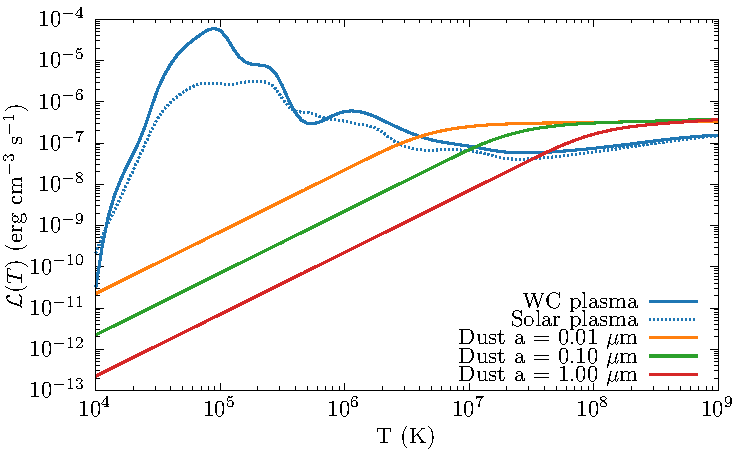
\includegraphics{assets/dust-plasma-cooling-comparison/cooling-comparison-forpaper2.pdf}
  \caption[Comparison of dust and plasma cooling rates in post-shock environment]{Comparison of energy loss due to plasma \& dust cooling with varying grain sizes in a typical post-shock flow, where $\rho_g = 10^{-16} \, \si{\gram\per\centi\metre\cubed}$ and a dust-to-gas mass ratio of $10^{-4}$. Whilst less influential at lower temperatures, dust cooling can aid cooling in the immediate post-shock environment.}
  \label{fig:postshockcoolcomparison-chapter3}
\end{figure}

% Difficulties in dust cooling integral, faster method of doing this

\begin{figure}
  \centering
  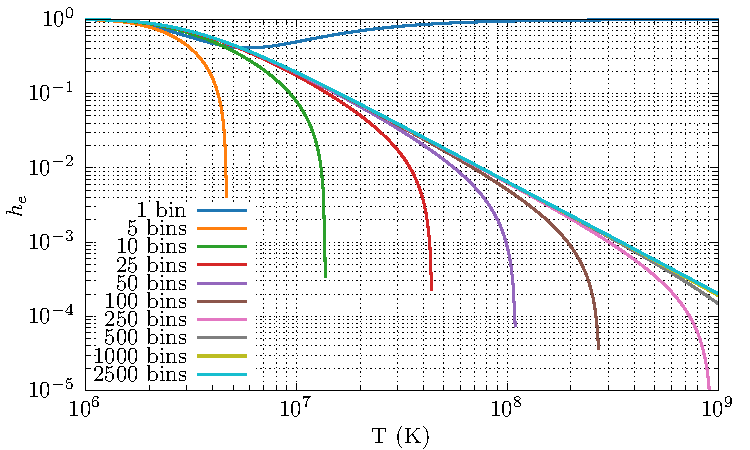
\includegraphics{assets/he_accuracy/he_acc.pdf}
  \caption[$h_e$ integration accuracy comparison]{Comparison of $h_e$ as a function of temperature for dust grains with a radius of 0.005 \si{\micro\metre}, $h_e$ is calculated via the trapezium rule with a varying number of bins, bin counts below 400 bins result in wildly inaccurate or in some case negative values for $h_e$, while beyond 400 bins the result is accurate and converges slowly.}
  \label{fig:he-accuracy-bins}
\end{figure}

Whilst a lookup table has proven to be adequate for plasma cooling, dust cooling for a given stellar wind is markedly more difficult to solve.
Whilst emissivity due to radiative processes in a gas or plasma can be parametrised in terms of temperature assuming that the flow abundances remain the same, the same does not apply to dust cooling, which requires three parameters, the grain radius, density and temperature.
Calculating emissivity due to dust is a markedly simpler proposition than calculating plasma emissivity, and could be performed quickly within a hydrodynamical code if only grain-atom interactions are considered.
Grain-electron interactions are a markedly more complex proposition.

The complexity in grain-electron interactions lies in determining the electron transparency, $h_e$, which is the probability that an electron will embed in the dust grain and heat it, rather than pass through.
$h_e$ can be computed via integration by parts, however due to this occurring in the main cooling loop, this results in a nesting of integrals, which can lead to extremely time-consuming computation for individual cells.
The integral could be simplified by reducing the number of bins to integrate with, however below approximately 400 bins the results can become extremely inaccurate, resulting in incorrect or even \textit{negative} values for $h_e$.
More complex integration methods reduce the number of steps required, but are in themselves more time consuming to calculate, leading to the same issue.
Initial tests using the integral method within a numerical simulation led to severe slowdown as processing time for cooling took up to 90\% of the overall processing time for each timestep.
The effect on grain heating due to electron interactions cannot be discounted, as it can be up to an order magnitude greater than grain heating due to incident atoms.
This was considered to be unacceptable in terms of performance, and as such a faster method needed to be determined.

Multiple options were considered for improving the performance of this routine.
Initially, a $\Lambda_d$ lookup table was considered, this consisted of a logarithmically spaced table of $\rho$, $a$, $T$ and $\Lambda_d$ values calculated by an implementation of the \cite{dwek_infrared_1981} prescription. 
A binary search for each parameter is performed, with the an offset, $P_d$, being calculated for each parameter,

\begin{equation}
  P_{d}=\frac{P-P_{0}}{P_{1}-P_{0}} , 
\end{equation}

\noindent
these offsets are then used to perform a trilinear interpolation to calculate $\lambda_d$ from the lookup table.

\begin{equation}
  \begin{split}
    \Lambda_{00} &=\Lambda_{000}\left(1-\rho_{d}\right)+\Lambda_{100} \rho_{d}, \\
    \Lambda_{01} &=\Lambda_{001}\left(1-\rho_{d}\right)+\Lambda_{101} \rho_{d}, \\
    \Lambda_{10} &=\Lambda_{010}\left(1-\rho_{d}\right)+\Lambda_{110} \rho_{d}, \\
    \Lambda_{11} &=\Lambda_{011}\left(1-\rho_{d}\right)+\Lambda_{111} \rho_{d}, \\
    \Lambda_{0} &=\Lambda_{00}\left(1-a_{d}\right)+\Lambda_{10} a_{d}, \\
    \Lambda_{1} &=\Lambda_{01}\left(1-a_{d}\right)+\Lambda_{11} a_{d}, \\
    \Lambda &=\Lambda_{0}\left(1-T_{d}\right)+\Lambda_{1} T,
  \end{split}
\end{equation}

%//TODO this needs a bit of sprucing, but makes sense
\noindent
where 0 is the lookup table value lower than the parameters actual value, and 1 is the lookup table value greater than the parameters actual value.
This implementation was written in the form of a series of nested loops to utilise SIMD vectorisation to improve performance.

% Further optimisations

Whilst this method is significantly faster than calculating $\Lambda$ for each cell with an integration step, a $(100 \times 100 \times 100)$ lookup table requires approximately \SI{32}{\mega B} of memory to store, and is much more time consuming to search through.
As such, eliminating complexity from the binary search and reducing the number of interpolations were identified as improvements to the 
These optimisations were made by simplifying the lookup table into a series of smaller lookup tables and relying on even logarithmic spacing of the lookup table to determine the parameter indices, rather than performing a binary search for them.
Additionally, as $\rho$ and $a$ are invariant within the cooling loop, these parameter offsets are solved separately using a bilinear interpolation, while in the cooling sub-step loop, a separate linear offset is performed to find the temperature offset, solving to find $\Lambda_d$. These optimisations resulted in this method scaling significantly better, as there is a lower total number of calculations required as the number of sub-steps increases (figure \ref{fig:dust-opt-speedup}).

\begin{figure}
  \centering
  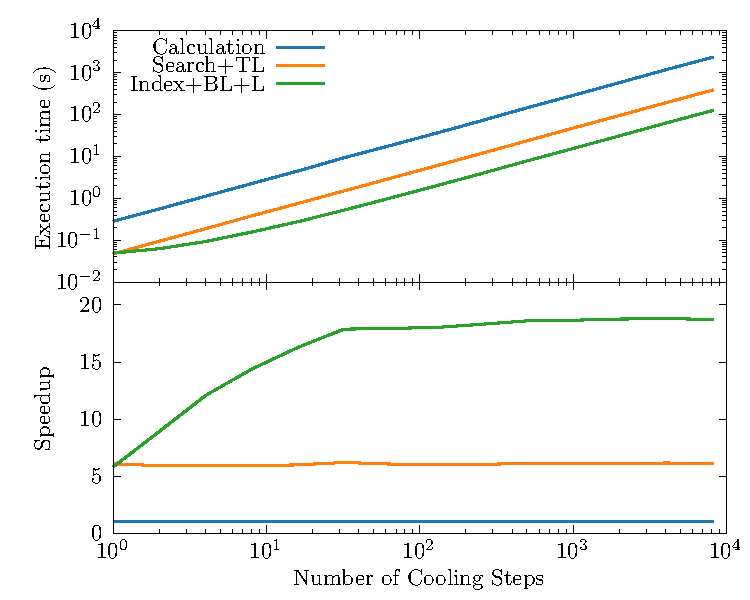
\includegraphics{assets/lambda-dust-speedup/lambda-dust-speedup.pdf}
  \caption[Dust lookup table methods comparison]{Comparison of execution time and speedup for lookup table methods.}
  \label{fig:dust-opt-speedup}
\end{figure}

% Approximation method 

The second method considered for solving the $h_e$ integral was using an approximation described by \cite{dwek_infrared_1981} where $h_e$ could be described by a series of equations:

\begin{equation}
  \begin{alignedat}{3}
    h_e(x^*) & = 1 ,                && ~~ x^* > 4.5, \\
    & = 0.37{x^*}^{0.62} , && ~~ x^* > 1.5 , \\
    & = 0.27{x^*}^{1.50} , && ~~ \text{otherwise,}
  \end{alignedat} \label{eq:electrontransparencyestimate}
\end{equation}

\noindent
where $x^* = 2.71 \times 10^8 a^{2/3}(\si{\micro\metre}) /T$.
Whilst this is less accurate, especially in the region where one case ends and the other begins where the result begins to diverge, this method is multiple orders of magnitude faster.
Figure \ref{fig:graintransacc} shows these discrepancies, in the case where electron transparency begins to decrease the approximation is out somewhat significantly, as well as mid-way through the curve, whilst at temperatures below $10^6 \, \si{\kelvin}$ the approximation and integral methods are perfectly aligned.
As the grains grow hotter and the electron transparency reduces, the influence on the cooling rate due to incident electrons reduces quite drastically, meaning that extremely high accuracy is less important at these temperatures (figure \ref{fig:contribution-int-vs-est}).
The accuracy of the approximation method is also shown in figure \ref{fig:lambda-comp-int-vs-est}, the estimated value for $\Lambda_d$ closely matches the integrated value aside from the smallest dust grains at very high temperatures $T>\SI{6e8}{\kelvin}$.

\begin{figure}
  \centering
  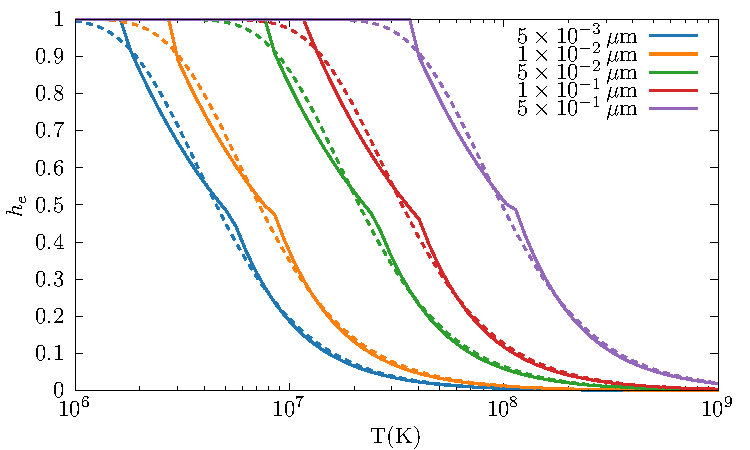
\includegraphics{assets/grain-transparency/grain-trans.pdf}
  \caption[Electron transparency method accuracy - $h_e$]{Grain transparency as a function of temperature for the estimate method described in equation \ref{eq:electrontransparencyestimate} (solid lines) and a 400 bin integration method (dashed lines).}
  \label{fig:graintransacc}
\end{figure}

\begin{figure}
  \centering
  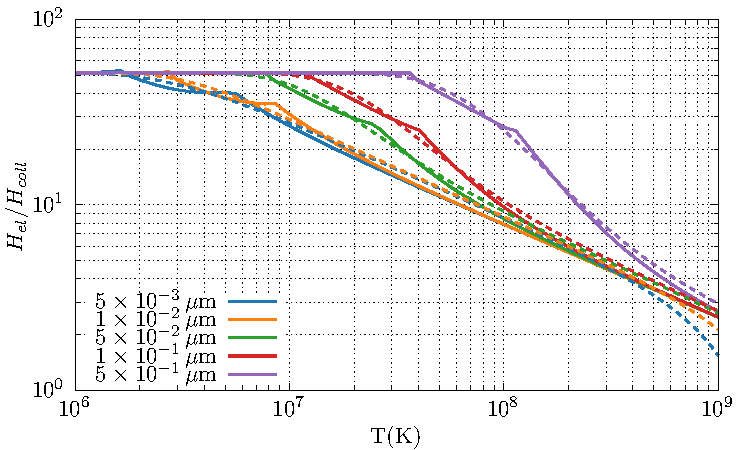
\includegraphics{assets/grain-transparency/contrib-comp.pdf}
  \caption[Electron transparency method accuracy - $H_{el}/H_{coll}$]{Comparison of the ratio heating rate of a dust grain due to incident electrons and incident atoms as a function of temperature for various grain sizes, whilst the result between the integration method and estimate method diverge, this is while the contribution of heating from electrons becomes less influential on the cooling rate of the grain.}
  \label{fig:contribution-int-vs-est}
\end{figure}

\begin{figure}
  \centering
  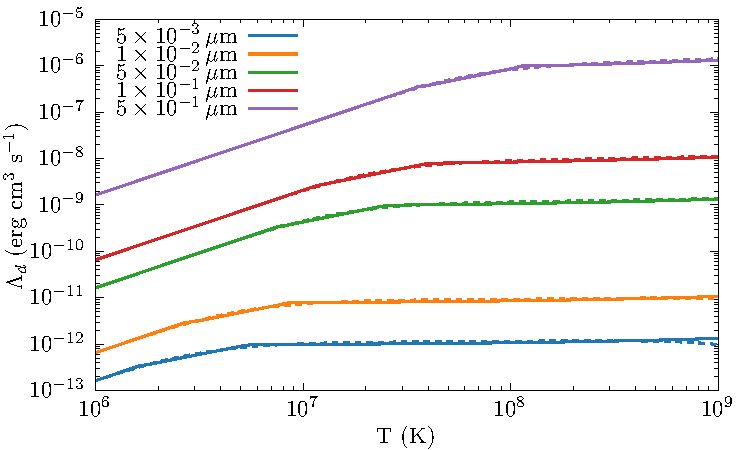
\includegraphics{assets/grain-transparency/lambda-comp.pdf}
  \caption[Electron transparency method accuracy - $\Lambda_d$]{$\Lambda_d$ as a function of temperature for various grain sizes, the estimate method is extremely close to the integral value aside from at the highest temperatures.}
  \label{fig:lambda-comp-int-vs-est}
\end{figure}

\begin{table}
  \centering
  \begin{tabular}{llll}
    \hline
    \multicolumn{1}{c}{\textbf{Method}} & \multicolumn{1}{c}{\textbf{t(s)}} & \multicolumn{1}{c}{\textbf{Iter/s}} & \multicolumn{1}{c}{\textbf{Speedup}} \\ \hline
    400 bin integration by parts & 36.03 & 35,526 & - \\
    Binary search + trilinear & 6.016 & 212,751 & 599\% \\
    Index calculation + bilinear + linear & 1.999 & 640,447 & 1,803\% \\
    \cite{dwek_infrared_1981} approximation & 0.147 & 8,693,171 & 24,510\% \\ \hline
  \end{tabular}
  \caption[Dust cooling calculation comparison]{Comparison of methods explored for estimating $\Lambda_d(\rho,a,T)$ in cooling code, $10^4$ initial values were chosen and 128 cooling sub-steps were performed, benchmark code was compiled and run using \texttt{GCC 10.3.0} with the \texttt{-O3} optimisation set on an Intel i7-7700HQ processor with a maximum clock speed of \SI{3.8}{\giga\hertz}.}
  \label{tab:electron-speedup}
\end{table}

% Compare accuracy and time taken
Table \ref{tab:electron-speedup} shows the improvements to performance inherent in the estimation method; the final result is that the approximation is over 24,500\% faster, the resulting dust cooling function therefore will have a minimal computational impact on the cooling loop as a whole.
As this approximation was conclusively shown to not significantly effect the cooling rate due to grain heating, the approximation was chosen.

Further improvements were made to correctly determine the electron number, $n_e$, to calculate the cooling contribution for dust due to grain-electron collisions.
the initial version of this code assumed that $n_e = 1.1 n_p$, an estimate based on solar abundances, however the electron-to-ion ratio varies significantly with temperature in a WC wind, which is hydrogen depleted and as such can vary from 0 to $\sim 4$ between \num{1e4} and \num{5e6} \si{\kelvin} (figure \ref{fig:electron-curve-no-elements}).
In order to solve this problem quickly for each timestep, a lookup table similar to the plasma cooling curves was used, containing the electron-ion ratio at temperatures between $10^4$ and $10^8$ \si{\kelvin} for each wind abundance.

\begin{figure}
  \centering
  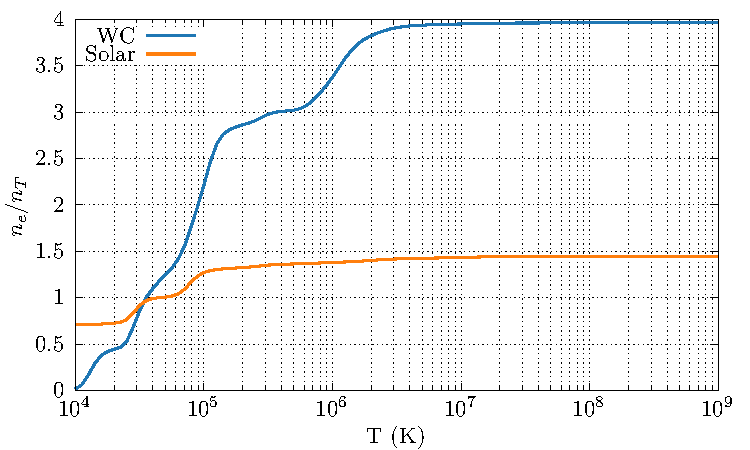
\includegraphics{assets/ionisation-fraction/ionisation-fraction-no-elements.pdf}
  \caption[Ionisation fraction for OB and WC stars]{Ionisation fraction}
  \label{fig:electron-curve-no-elements}
\end{figure}

%%//FIXME cooling loop schematic!

% Something along the line of This schematic describes, etc. etc. 
% Schematic

\subsection{Implementation}
\label{sec:cooling-implementation}

In order to simulate energy loss due to radiation in Athena++, the conserved variable array is adjusted to remove energy from a specific cell, this is analogous to energy being removed from the system due to radiative processes.
This process is assumed to be 100\% efficient, re-adsorption and scattering is not simulated, as this would be very complex to simulate at every time step.

% Flesh out cooling problem in general 

Radiative processes are part of a source function that is performed for every mesh block.
The cooling routine within the source function iterates through all cells within the meshblock, calculating radiative energy loss for each cell.
% Lookup table method recap + how it is applied
Within the loop, the cell parameters are loaded from the conserved variables array, and additional gas and dust parameters are calculated from these conserved variables.
in particular the mean molecular mass of a cell is calculated with the formulae:

\begin{equation}
  \mu = C\mu_{WR} + (1-C) \mu_{OB}, \label{eq:windaveraging}
\end{equation}

\noindent
where $\mu_{WR}$ and $\mu_{OB}$ are the mean molecular masses of the winds and $C$ is the wind ``colour'' scalar, the contribution of each wind to the gas density of the cell.
The temperature is subsequently calculated using the ideal gas law:

\begin{equation}
  T = \frac{P \mu m_H}{\rho k_B}.
\end{equation}

\noindent
At the current temperature, the cooling parameter, $\Lambda(T)$ for each wind is found from the lookup tables, and weighted in a similar manner as equation \ref{eq:windaveraging}. The energy loss due to dust grains is then calculated, with the total energy loss rate within the cell defined as:

\begin{equation}
  \dot E = \dot{E}_\text{G} + \dot{E}_\text{D} = \left(\frac{\rho}{m_H}\right)^2 \Lambda_\text{G}(T) + n_\text{D} \dot{E}_\text{grain},
\end{equation}

\noindent
this energy loss rate is then multiplied by the timestep, $dt$, and then subtracted from the total energy within the cell. 

% Timestep method, why is this used rather than a single timestep

One of the main issues with estimating the cooling rate rather than performing an exact calculation of energy loss is that the cooling rate and current temperature are coupled, this can result in wildly inaccurate final temperatures at the end of the cooling step compared with an exact integration.
This is especially a concern at the expected temperatures in the post-shock, radiatively cooled environment, as the $\Lambda(T)$ is maximised at approximately $10^5$ \si{\kelvin}. If the timestep is too large this can result in over-estimation of the cooling.
The simplest solution would be to make the time-step smaller, however this would reduce the performance of the code, as the cooling loop takes significantly less time to perform than the hydrodynamical loop.
Instead, adaptive sub-stepping is used to iterate through the time-step, adjusting the maximum sub-step for an integration based on the current gas parameters, specifically the amount of energy remaining in the cell.
Figure \ref{fig:cooling-loop-evolution} shows the adaptive sub-stepping routine in operation, at the initial time, the cooling parameter $\Lambda$ is maximised, as such the time-step is significantly lower than when the gas has cooled as is less radiative.
This compares favourably to a single sub-step example, which would cause the simulation to crash due to negative temperatures, and with linearly spaced steps, which either required many more steps or were potentially unstable.

\begin{figure}
  \centering
  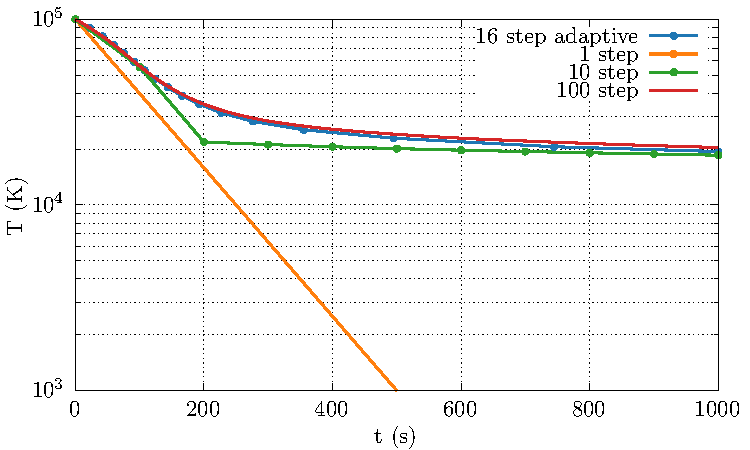
\includegraphics{assets/plasma-cooling-benchmarks/evolution.pdf}
  \caption[Cooling sub-step method evolution comparison]{Comparison of the adaptive timestep method versus linearly spaced sub-steps for a solar abundance flow with a density of $10^{-16}$ \si{\gram\per\centi\metre\cubed} and an initial temperature of $10^5$ \si{\kelvin}.}
  \label{fig:cooling-loop-evolution}
\end{figure}

A suitably accurate maximum cooling time is calculated by first calculating the cooling time in the cell using the formulae:

\begin{equation}
  \tau_\text{cool} = \frac{E_i}{\dot{E}_\text{iter}},
\end{equation}

\noindent
where $E_i$ is the cells internal energy and $\dot{E}_\text{iter}$ is the total energy loss rate for the current iteration.
A fraction of this value is used as the sub-timestep, which is used to calculate the energy loss in that iteration.

\begin{equation}
  dt_\text{step} = \kappa \tau_\text{cool}, \label{eq:kappafirstuse}
\end{equation}

\noindent
Another iteration of the cooling calculation is then performed, with sub-step time re-calculated, until the elapsed time is equal to the hydrodynamical timestep, $dt$. Throughout the simulations in this project a value of $\kappa = 0.1$ was adopted.

In order to assess the performance and accuracy of this method, a test environment was produced to simulate the radiation of a region of gas in the post-shock environment.
For this test, a gas density of $10^{-16}$ \si{\gram\per\centi\metre\cubed} and an integration timestep of \SI{1000}{\second} were utilised.
In order to demonstrate the flexibility of the adaptive method over the temperature ranges of a CWB simulation, initial temperatures of $10^5$, $10^6$ and $10^7$ \si{\kelvin} were used to demonstrate the models effectiveness in the cool, warm\footnote{See what I mean about the phrase ``warm''?} and hot regimes of the WCR.
This was compared with the exact integration method proposed in \cite{townsendExactIntegrationScheme2009} as well as a modified version of the cooling code which uses evenly spaced sub-steps. To demonstrate the relative accuracy of the chosen cooling timescale fraction, lower values of $\kappa$ were also used to demonstrate that lower values, while more accurate, were much more computationally complex.

% Discuss results of benchmarking

% Potential other methods, such as using an RK solver or more through adaptive timestep
The main limitation of a first-order Euler integration method such as this is that it converges on the correct answer slowly, and as such will be out by a few percent in the worst case so long as a sensible sub-step is used.
Table \ref{tab:cooling-loop-speed-comp} shows that while an iteration of the logarithmic index method used in this project is slightly more performant than the fast exact integration method proposed in \cite{townsendExactIntegrationScheme2009}, multiple sub-steps quickly render this performance benefit moot, in high-temperature cases with a lower gas density this method is much more accurate with fewer steps, however, as such this method was considered suitable for performing radiative cooling in the high-temperature immediate post-shock environment and lower density low-temperature WCR environment, where the bulk of this project focusses.

%//TODO plot to compare accuracy compared to single step, adaptive substep and arbitrarily large number of timesteps, temperature initial temperature 10^5K and density 10^-16g/cm^3, show tfloor as well

\begin{figure}
  \centering
  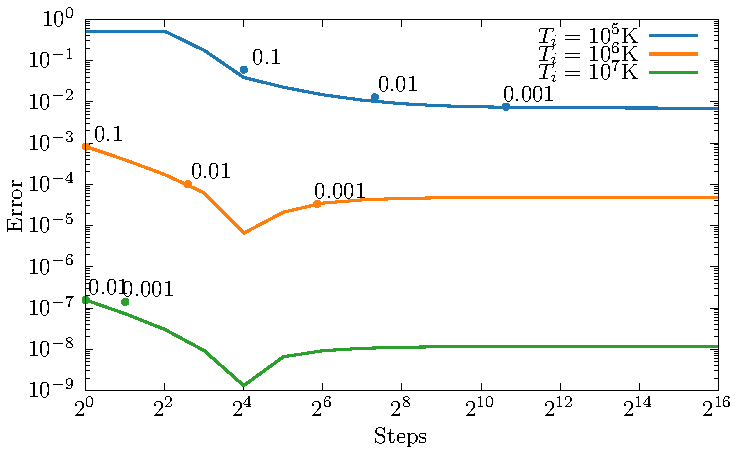
\includegraphics{assets/plasma-cooling-benchmarks/convergence.pdf}
  \caption[Cooling sub-step method accuracy comparison]{Comparison of estimated , points represent $\kappa$, in the low temperature case the answer is not particularly accurate, but with the adaptive method with $\kappa = 0.1$ the result is only out by a few percent for a small number of sub-steps.}
  \label{fig:cooling-loop-convergence}
\end{figure}



\begin{table}[h]
  \centering
  \begin{tabular}{ccccccc}
  \cline{2-7}
   & \multicolumn{2}{c}{$\kappa = 0.1$} & \multicolumn{2}{c}{$\kappa = 0.01$} & \multicolumn{2}{c}{$\kappa = 0.001$} \\ \hline
  $T_i$ & Steps & Error & Steps & Error & Steps & Error \\
  $\SI{1e5}{\kelvin}$ & 16 & \num{6.025e-02} & 159 & \num{1.282e-02} & 1585 & \num{7.637e-03} \\
  $\SI{1e6}{\kelvin}$ & 1 & \num{8.233e-04} & 6 & \num{1.012e-04} & 58 & \num{3.359e-05} \\
  $\SI{1e7}{\kelvin}$ & 1 & \num{1.577e-07} & 1 & \num{1.577e-07} & 2 & \num{1.411e-07} \\ \hline
  \end{tabular}
  \caption[Cooling method accuracy comparison]{Accuracy of the adpative sub-step Euler method compared with the \cite{townsendExactIntegrationScheme2009} exact cooling method, with $\kappa = 0.1$ this method is out by $6\%$ at worst in the low-temperature example, while very accurate at higher temperatures with only a single step needed.}
  \label{tab:cooling-loop-accuracy-comp}
\end{table}

\begin{table}
  \centering
  \begin{tabular}{cccc}
  \hline
  & \textbf{Search} & \textbf{Logarithmic} & \textbf{\cite{townsendExactIntegrationScheme2009}} \\ \hline
  $\tau$ (\si{\nano\second}) & 146 & 134 & 151 \\
  $\Delta \tau$ (\si{\nano\second}) & 8.0 & 1.5 & 0.9 \\ \hline
  \end{tabular}
  \caption[Cooling method performance comparison]{Comparison of performance between first order Euler integration methods and the exact integration method described by \cite{townsendExactIntegrationScheme2009}. Tests were conducted with a sample of $10^6$ iterations on a 3.2 \si{\giga\hertz} M1 processor, while the code was compiled using \texttt{clang 12.0.5} and the \texttt{-O3} optimisation set.}
  \label{tab:cooling-loop-speed-comp}
\end{table}

Whilst this is a fairly simplistic method of performing adaptive sub-stepping, it is fast, effective, and not prone to failure. An adaptive RK method and implicit method were also considered, but not utilised in the final code, as this sub-stepping procedure was intended for speed and numerical safety over accuracy.

% Unresolved interfaces, need to elaborate

Care is made to correctly calculate energy loss around unresolved interfaces. \textit{Finish this!}

%//TODO need to ask Julian how this is done

% Wrap up, how can this method be improved in general, more exact solvers, what would be the ideal?

\section{The BODMAS Advected Scalar Dust Model}
\label{sec:bodmas}

Binary Orbit Dust Model with Accretion and Sputtering\footnote{All good theses have a laboured acronym!}

The primary focus of this project was to implement a dust model within a numerical simulation, in order to determine the growth of dust grains within the 

\subsection{BODMAS features}

\subsection{Implementation}

The most processing efficient method of 

% Co-moving, drawbacks in general

This method does have its drawbacks, principally, the advected scalar method cannot simulate grain-grain or grain-gas interactions with high relative velocities, such as interactions within the wind collision region, where 

\subsection{Contemporary dust Models}

% Ballistic dust model

% Numerical dust models in non-cwb systems?

\subsubsection{The Hendrix dust model}

Perhaps the most similar contemporary dust model is the model described in \cite{hendrix_pinwheels_2016} - as this model is concerned with simulating the dynamics of dust within a CWB.
This is not to say that these models are identical, of course, as the Hendrix model explores how dust spreads throughout the WCR of WR 98a, in order to compare with observational data using radiative transfer code.
%//FIXME double check that one king 

% Differences between models 

The main differentiating factors between this model and our model are the driving mechanism and dust evolution.
In the Hendrix model dust is modelled as a separate fluid, with an Epstein drag function between the wind and dust fluids; this method allows for dust kinematics that aren't implicitly co-moving.
This is a more accurate method of modelling dust, however it requires significantly more processing time and is much more difficult to implement, requiring a numerical code that supports multiple fluids.
At the start of this PhD this was considered but eventually rejected due to time constraints.

However, the Hendrix model has limitations that this model does not have, this is because the purpose of the Hendrix model is to analyse the distribution of dust within a CWB system, rather than to model the evolution of the dust itself.
To this end, the Hendrix model does not calculate dust growth or destruction, and only uses a single small grain size, with the dust-to-gas mass ratio calculated based on observations of the target system, WR98a.



\subsection{Future dust models}

% Future work, adopt multi-fluid model?

Due to time constraints and limitations in the code in use, only a limited set of mechanisms for dust evolution were included in this projects simulations.
While the BODMAS model represents an interesting start for the modelling of dust grains in colliding wind binaries, future models could implement more complex models which incorporate additional destruction and growth mechanisms as well as 

A multi-scalar model could be used to more accurately measure the growth of dust grains, rather than a single average grain size and 
This would be more difficult to implement than a single model but would be able to simulate the growth of grains with a large number 
Athena++ and MG both have issues with a large number of scalars, as such both numerical codes may require significant modification to cope with this.
A multi-fluid model with dust being physically simulated rather than assumed to be perfectly co-moving would be an ideal next step.
Multiple grain size distributions could also be modelled in a similar way to the proposed multi-scalar model, however the kinematics of the dust grains could also be simulated separately.
% Mixing factors
The increased inertia of more massive dust grains could result in the kinematics of the dust flow diverging from the co-moving assumption.
To that end, a successor dust model would adopt a multi-fluid and drag function method, which was considered but not included for the sake of time.
This multi-fluid model would also allow for more physically accurate simulation of grain-gas and grain-grain interactions, as the collision velocities would be exactly calculated rather than estimated through bulk motion properties, high speed collision of gas on dust grains in the immediate post-shock environment could also shatter grains, though modelling this as well as spalling of particles in the wind through the dust grains would be complex to simulate. 

Furthermore, additional mechanisms for dust destruction, such as through photodissociation and sublimation could also be implemented, the implementation of these could be used to determine the effectiveness of the WCR in protecting nascent, still forming dust grains.

% Better dust nucleation model
% //TODO this section needs work

The initial grain nucleation model could also be improved, injection of extremely small grains into the simulation through the stellar remap zones was chosen as the underlying chemical process for formulation of these dust grains is poorly understood at the time of writing.
% Current model not too bad, strong dependence on a but z does not change much, being dependent on a single parameter not too bad
The small grain nucleation model was also found to be only dependent on the initial grain radius, $a_i$, whilst changing the amount of grain nuclei in the WR wind does not change the amount of dust produced.
As such the simulations are currently bound by a single input parameter, which can be constrained based on what is currently understood about dust grain accretion.
% Difficulty in picking initial parameters for more complex model
A more complex model may require additional parameters, and as such would be highly dependent on them.

% Comparison with observational results

Another avenue of future research would be performing a radiative transfer simulation upon a fully advected system, in order to compare with 
This was initially considered at the start of the project, but was not performed due to the limited amount of time remaining at the end of the PhD.
This was performed by \textcite{hendrix_pinwheels_2016}, with the resultant images emulating the sensitivity and angular resolution characteristics of UKIRT, Keck and ALMA (figure \ref{fig:hendrix-synthetic}).
Radiative transfer models would be used to 

\begin{figure}
  \centering
  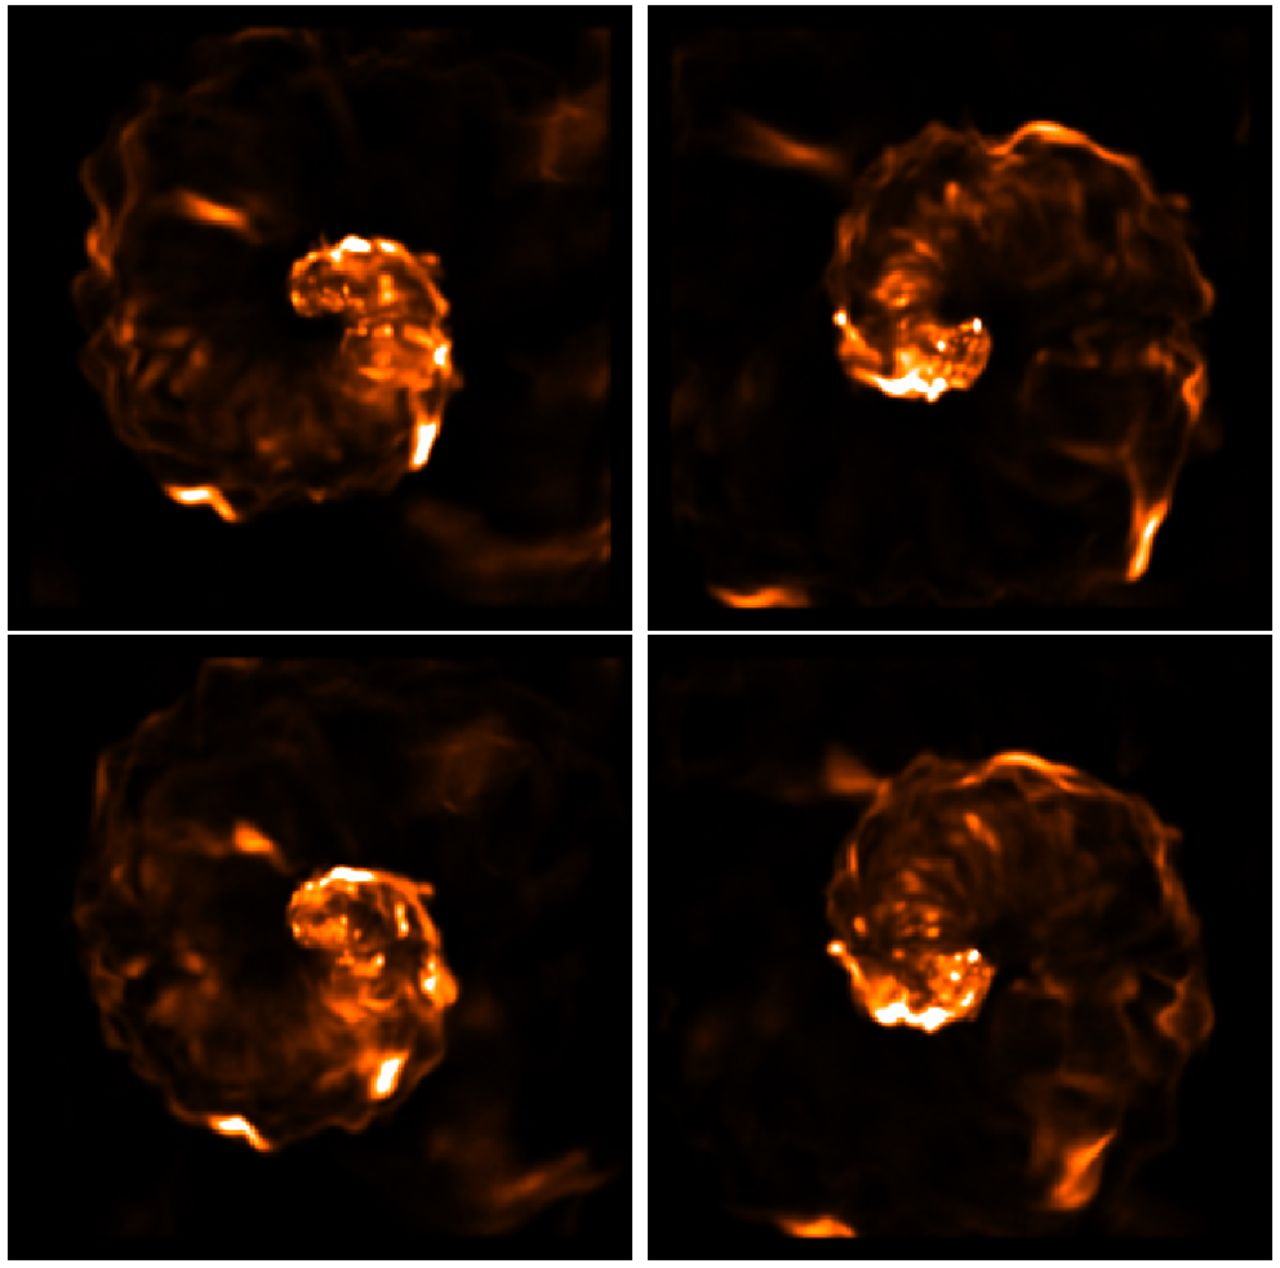
\includegraphics{assets/hendrix-synthetic-observation.jpeg}
  \caption[\textcite{hendrix_pinwheels_2016} synthetic astronomy]{Synthetic images of WR 98a emulating the capabilities of ALMA using a radiative transfer model, reproduced from \textcite{hendrix_pinwheels_2016}.}
  \label{fig:hendrix-synthetic}
\end{figure}